\chapter{Case study: Pollution-aware user navigation}
\label{chap:case-staudyLoRa}

This chapter presents the case study used as reference scenario during the evolution of the DingNet simulator, and to evaluate the limits of communications from applications to LoRa motes. 
A demo from this case study was showed during the Day of Science in Flanders to present the LoRaWAN technology receiving a lot of attention.

\section{Case study description}
Leuven is a cycling city where most of the inhabitants and students use daily their bike to move across the city. 
In this context we want to realize a system able to provide to the user the healthiest route to reach a destination. 
The route generation will be based on the air quality level, based on the CAQI index~\cite{CAQI}, of the crossed areas to reach the destination. 
The user, in order to obtain the route, has to require it to the application deployed in a remote server.
The system uses data received from the sensor network to create a city map of quality air.
Then, the application has to define the route to a destination that optimize the trade-off between air quality and length of the route.
The system should be able to recompute the best route if the environment condition change, and communicate it to the user.
The sensor network can be composed by two types of sensors:
\begin{itemize}
    \item \textbf{Fixed}: positioned along the roads and at intersections
    \item \textbf{Mobile}: placed on public transport or bicycles
\end{itemize}
All the sensors have to be deployed in a LoRaWan network.
Similarly also the user device, which interacts with the application to require the route, has to use the LoRa technology.

\section{Design of the system}
\autoref{fig:caseStudyA} shows the high level architecture of the system, and introduces the main entities. 
The main entities are the sensors devices, the user devices, and the routing application.
As requirement both sensors devices and user devices have to be displaced inside the LoRaWAN network and use the LoRa technology to communicate with the routing application.
Using the DingNet simulator to simulate the LoRaWAN network:
\begin{itemize}
    \item the routing application is mapped in a generic application deployed in the application server that communicates with the LoRaWAN network via MQTT
    \item the sensor devices, which have to send only packet with the sensed value, can be mapped in the \textit{Mote} simulator entity
    \item the user devices are special devices, because they do not send only packets with the sensed value. They have also to require the route for a destination and be able to manage the received packets with the route. Actually there is not simulator entity with this specific abilities, so it will be necessary to define it.
\end{itemize}
% 
\begin{figure}[h]
    \centering
    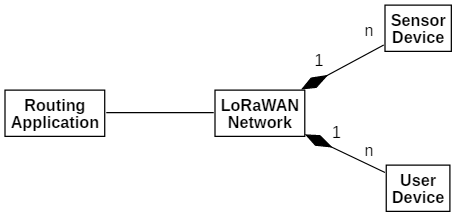
\includegraphics{figures/CaseStudyA_HLarch.png}
    \caption{High level architecture of the system}
    \label{fig:caseStudyA}
\end{figure}
% 
\subsection*{Interaction between application and devices}
If on one hand the transmissions from the devices (both sensor and user) to the application are in compliance with the maximum packet's length defined by the LoRaWAN standard (1 byte for packets with the sensed value, and 16 bytes for the packet to require the route); on the other hand it is impossible to send the packet from application to the user device with the entire route, so the only way to do it is to split the packet.
In order to send the entire route to the user device, two approaches are available: 
\begin{enumerate}
    \item define a specific interaction protocol to send all the packets with the entire route to the user device immediately after its computation
    \item send a packet with part of the route only when the user has finished the previous part of the route.
\end{enumerate}
Considering also the requirement to recompute the route if the environment condition change, the second option is chosen, enabling to recompute the route before send its next part.

\subsection*{Design of the user device}
% UserMote - consume packet
The user device has to perform three activity: require the route, send update of its position, and manage the incoming packets.
If on one hand the last two activity can be performed also from a \textit{Mote}, on the other hand it cannot require the route.
For this reason in \autoref{fig:userMote} a new entity simulator is introduced, the \textit{UserMote}. 
It extends the \textit{Mote} adding the logic to require the route when needed sending a packet with starting and destination positions.
Then to manage incoming packets are chosen \textit{MaintainLastPacket} as strategy to store them until that they are consumed, and \textit{ReplacePath} as only strategy to consume them.
It consumes each packet updating the user route in accord with the packet payload until the route is completed.
To perform the last activity, send updating of the user position, is only necessary add the GPS sensor to the \textit{UserMote}, and send it when the user is closer to the sub-route destination.
% 
\begin{figure}[h]
    \centering
    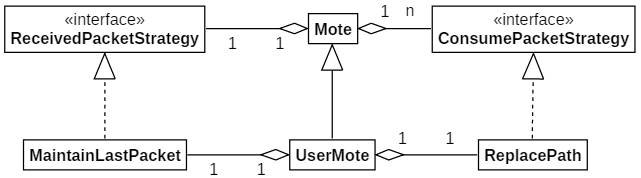
\includegraphics{figures/userMote.png}
    \caption{\textit{UserMote} model.}
    \label{fig:userMote}
\end{figure}
% 

\subsection*{Routing application}
The application to found the best route implements an A-star algorithm on the graph of street of the city. 
The weight of the edges of the graph corresponds to the distance between the two points multiply for a factor that represents the air quality level in that street. 
The values sensed by the sensors are retrieved subscribing the topics where the LoRaWAN network publishes them. 
The route is sent to the user mote publishing the massage with sub-route on its receiving topic.
The application recomputes the best route only when the user device communicates its new position and if some environment condition is changed from the previous computation.

\section{Simulation in DingNet}

This section presents the simulations of two possible small scale scenarios. 
The simulations are conducted over the city of Leuven with the DingNet simulator.
First, the setup of the two simulated scenarios is presented; then the simulation results discussed in a qualitative way based on simulation snapshots.

\subsection{Setup}
Both the scenarios present a common configuration and differ only for the starting position of the user.
The environment is composed of:
\begin{itemize}
    \item 2 gateways
    \item 4 fixed sensors equipped with a set of sensors and send directly the final CAQI index value.
    \item one mobile sensor that follows a path like a public transport. It assume the same behaviour of a fixed sensor, but is equipped also of a GPS sensors.
    \item user that requires a route to a destination.
\end{itemize} 
All the types of LoRa devices are configured in a way to try to reduce collision between transmissions.
In the first scenario the user start from the south of the city, which is the most polluted in the simulation configuration; while in the second scenario the user starts from the north of the city.

\subsection{Result}

\autoref{fig:sim1} and \autoref{fig:sim2} show snapshots taken from the two simulated scenarios.
The transparent layer represents the air quality level in that point based on the received sensor value.
The mote number 4 is the mobile sensor and the red line is its route.
The user is identified by the cyclist. 
Its line (route) is of two colors: blue and red.
The blue one is the complete route computed by the application, while the red one is the sub-route received by the user until that time. 

\autoref{fig:sim1} shows three snapshots of the first simulated scenario.
First snapshot shows the initial situation and the first computed route.
Second snapshot shows how after an environment conditions change, the route is recomputed with a longer one, but considered better by the application, combining distance with pollution. 
So the user has received a new sub-route of the new best route that starts from its actual position.
Finally, the last snapshot shows the user arrived to destination.
% 
\begin{figure}[h]
    \centering
    \begin{tabular}{lll}
         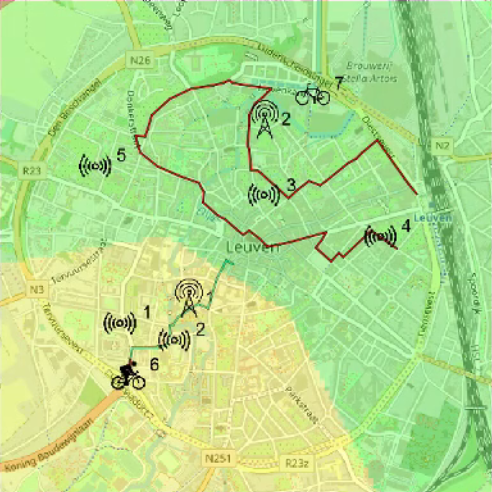
\includegraphics[scale=0.42]{figures/sim1snap1.png}  &
         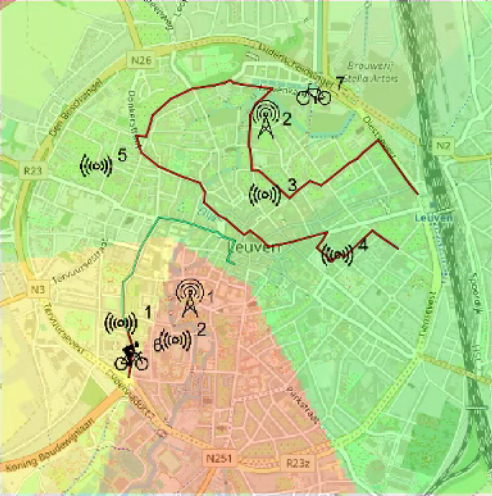
\includegraphics[scale=0.42]{figures/sim1snap2.png} &
         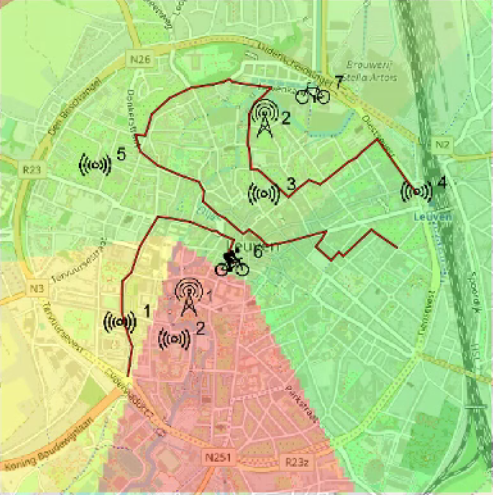
\includegraphics[scale=0.42]{figures/sim1snap3.png} 
    \end{tabular}
    \caption[Three snapshots of a simulation run with changing of the route]{Three snapshots of a simulation run with changing of the route dues to the change of the environment conditions.}
    \label{fig:sim1}
\end{figure}
% 

\noindent \autoref{fig:sim2} shows three snapshots of the second simulated scenario.
In this case the user best route never changes because the change of the environmental conditions do not affect the areas crossed by him.
% 
\begin{figure}[h]
    \centering
    \begin{tabular}{lll}
         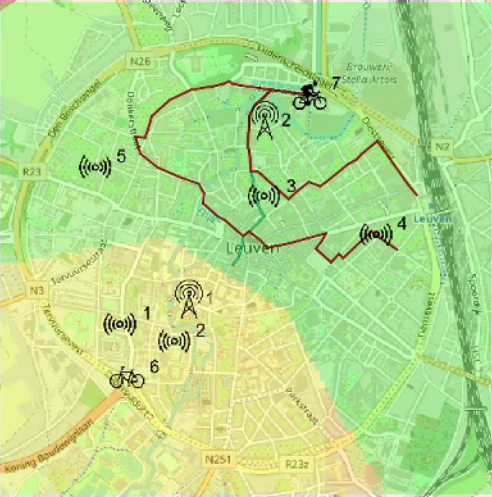
\includegraphics[scale=0.42]{figures/sim2snap1.png}  &
         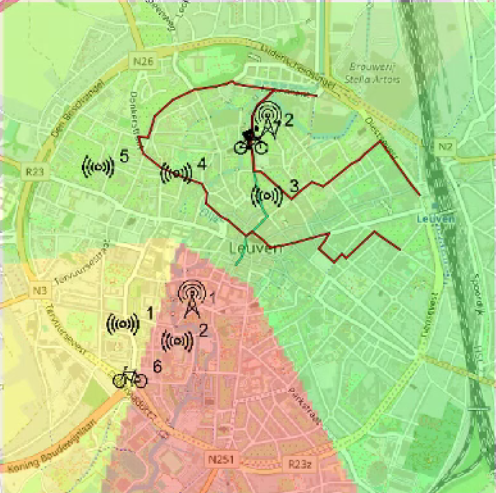
\includegraphics[scale=0.42]{figures/sim2snap2.png} &
         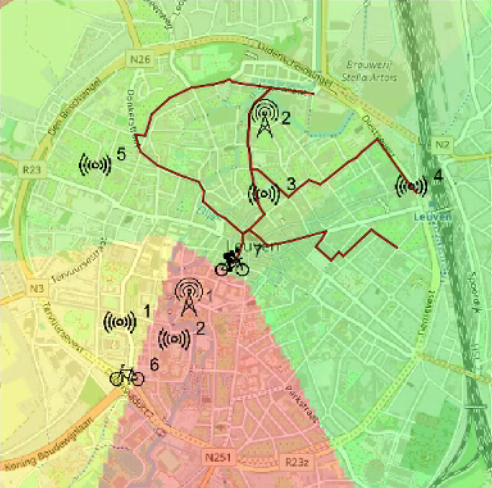
\includegraphics[scale=0.42]{figures/sim2snap3.png} 
    \end{tabular}
    \caption[Three snapshots of a simulation run without changing of the route]{Three snapshots of a simulation run without changing of the route despite the change of the environmental conditions.}
    \label{fig:sim2}
\end{figure}
% 

Although they are simple simulations with few sensors and only one user device, it can be deduced that use LoRa technology also for user devices is possible only in certain scenarios.
In these scenarios the number of transmissions necessary to transmit all the route is high, so according to LoRaWAN limitations it is possible only for short route.
Moreover considering a real scenario where the number of user is higher (es. more than one thousand) the network congestion will increase with also the probability of collisions among transmissions, which require re-transmission worsening the situation.

\paragraph{Concluding.} This chapter has presented the case study used as reference for the simulator evolution.
It has helped to consider the behaviour of all the network facilities and the bi-directional communication schema.
It has confirmed the validity of LoRaWAN as enabling technology for a sensor network and its limits regarding the communication from application to LoRa devices.